\section{Concentration Dependent Reaction}
	
	In this section we consider the reaction as a concentration dependent quantity. This is
	
	
	\begin{align}
		J_{x=0} = -D\frac{\partial C}{\partial x}\big|_{x=0} = -R,
	\end{align}
	
	where $R$ is given by the Langmuir absorption model \cite{langmuir}
	
	\begin{align}
		R = \frac{k_fC(0, t)}{1 + K_{eq}C(0, t)},
	\end{align} 
	
	where $k_f$ is a constant proportional to the number of available sites in the solid surface and  and $K_{eq}$ is the equilibrium constant of the reduction of copper reaction at the interface.
	
	If $K_{eq} << k_f$, we can expand this into what is known as the Freundlich formula,
	
	\begin{align}
		R \approx k_f C(0, t),
	\end{align} 
	
	with $k_f = k/K$. For this case, we get the following boundary condition for the flux
	
	\begin{align}
		J_{x=0} = -k_fC(0^+,t),
	\end{align}
	
	which yields a Robin type of boundary condition for our system
	
	\begin{align}
		 \frac{\partial C}{\partial x}\big|_{x=0} -\frac{k_f}{D}C(0^+,t) = 0.
	\end{align}
	
	Thus, we need to solve the following system
	
		
	\begin{align}
		\frac{\partial C}{\partial t} = D \frac{\partial^2 C}{\partial x^2},
		\label{eq:dynamic-system-langmuir}
	\end{align}
	
	\begin{align}
		C(x = \delta, t) =& C_b,\\
		\frac{\partial C}{\partial x}\big|_{x=0} -\frac{k_f}{D}C(0^+,t) =& 0,\\
		C(x, t=0) =& 0.
		\label{eq:boundary-conditions-dynamic}
	\end{align}



The diffusion equation for this set of boundary conditions is solved in detail in Appendix \ref{appendix:analytic-langmuir}





\begin{figure}[htbp]
\centering
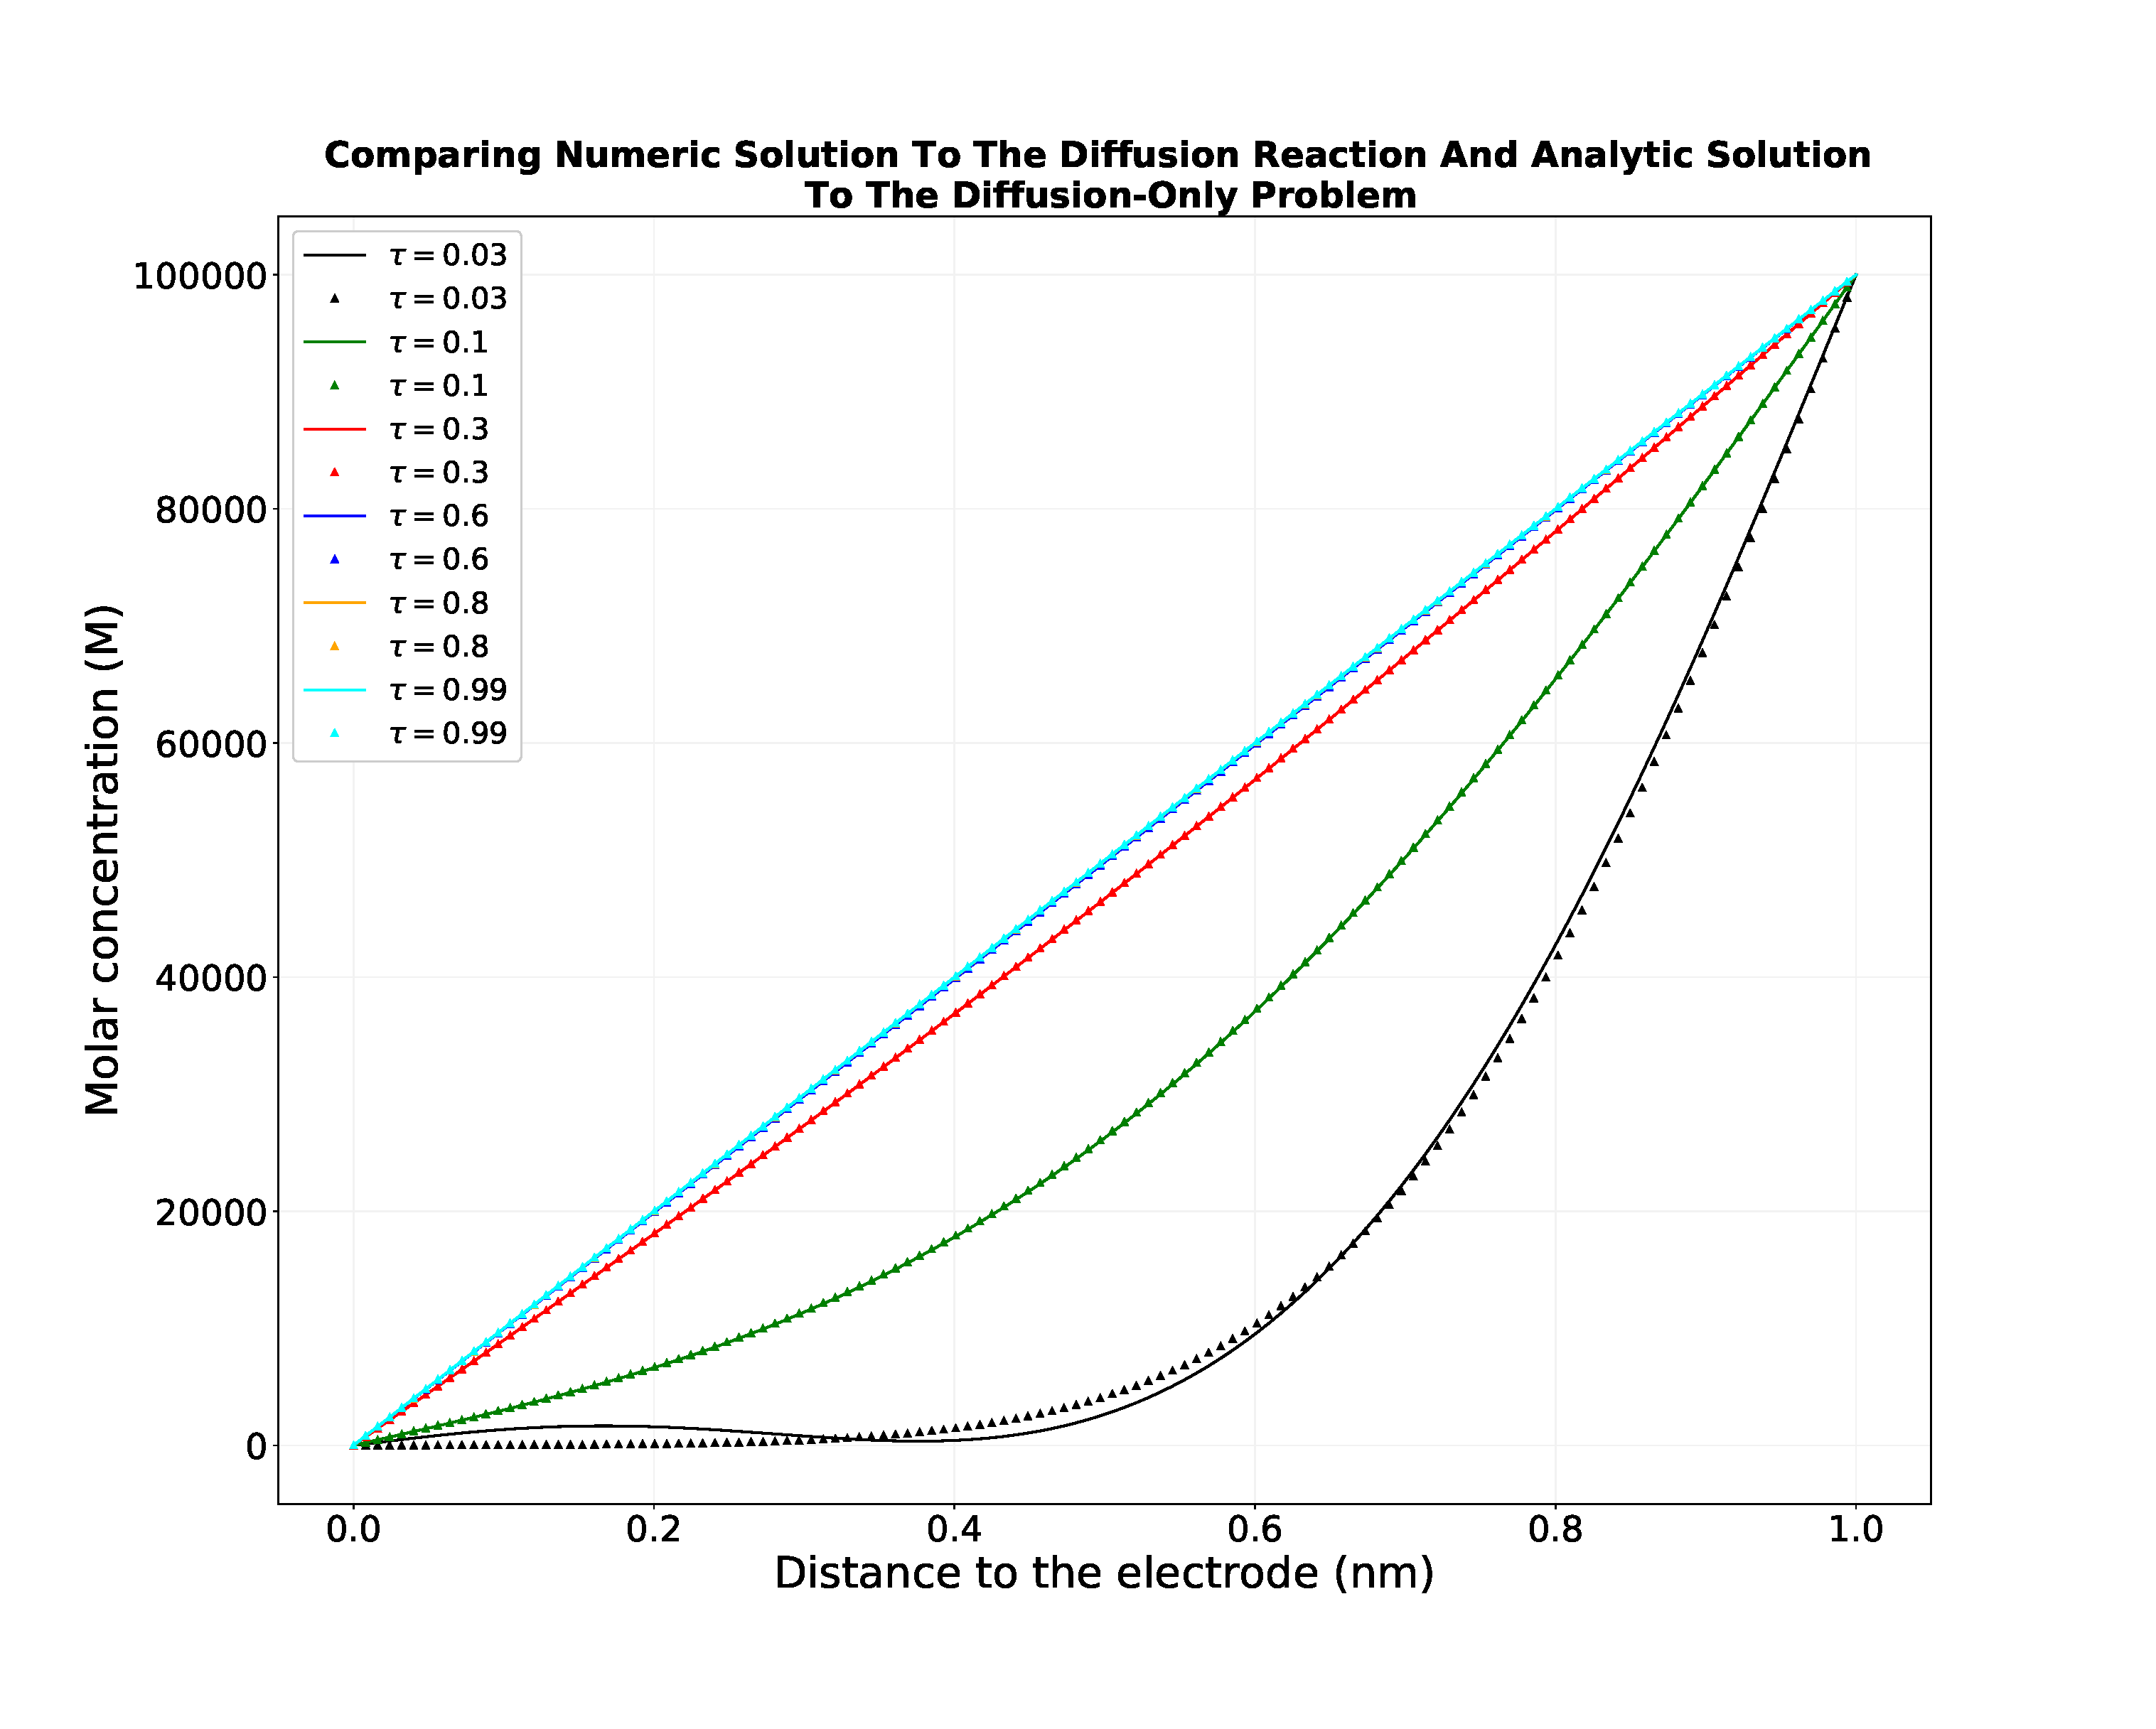
\includegraphics[width=\textwidth]{concentration-diffusion-reaction-robin-comparison}
\caption{In this model, the boundary conditions are physically sensible as the depend on charge carriers to arrive at the interface to produce current. At small $t$ there is no current as copper ions have not reached the surface at $x-0$ and it increases linearly with concentration as time goes on.}
\label{fig:diffusion-reaction-comparison}
\end{figure}

\newpage